\documentclass[tikz,border=12pt]{standalone}
\usepackage[T1]{fontenc}
\usetikzlibrary{calc}
\begin{document}
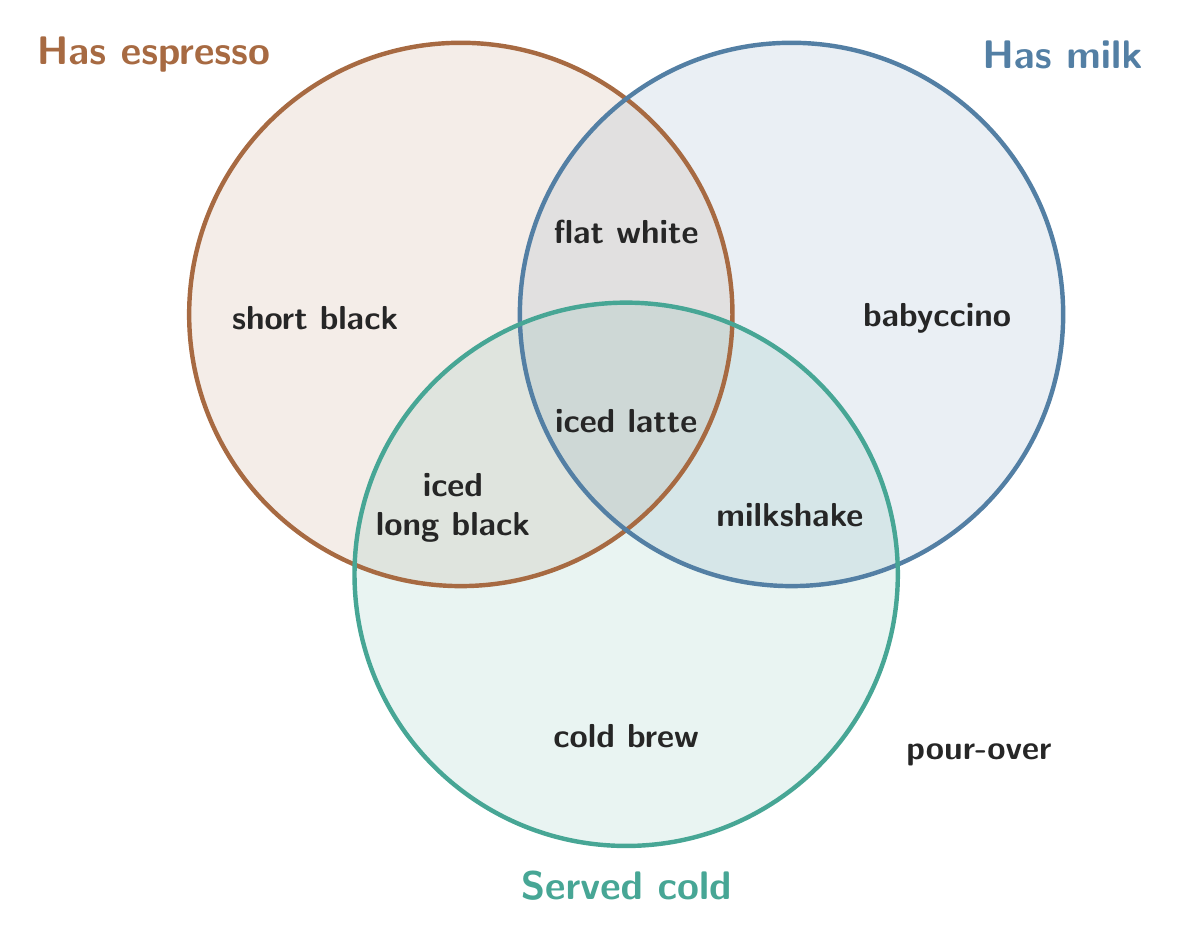
\begin{tikzpicture}[font=\sffamily]
  % Sets: espresso (left), milk (right), cold (bottom).
  \definecolor{espresso}{HTML}{A76A42}
  \definecolor{milk}{HTML}{537FA4}
  \definecolor{cold}{HTML}{47A695}
  \coordinate (E) at (-2.1,1.3);
  \coordinate (M) at ( 2.1,1.3);
  \coordinate (C) at ( 0,-2.0);
  \def\r{3.45}
  \fill[espresso,opacity=.12] (E) circle (\r);
  \fill[milk,opacity=.12] (M) circle (\r);
  \fill[cold,opacity=.12] (C) circle (\r);
  \draw[espresso,line width=1.6pt] (E) circle (\r);
  \draw[milk,line width=1.6pt] (M) circle (\r);
  \draw[cold,line width=1.6pt] (C) circle (\r);

  \tikzset{drink/.style={align=center, text=black!85, font=\sffamily\bfseries\large}}
  \node[drink] at (-3.95,1.25) {short black};
  \node[drink] at ( 3.95,1.25) {babyccino};
  \node[drink] at ( 0,2.35) {flat white};
  \node[drink] at (-2.20,-1.15) {iced\\long black};
  \node[drink] at ( 2.08,-1.25) {milkshake};
  \node[drink] at ( 0,-.05) {iced latte};
  \node[drink] at ( 0,-4.05) {cold brew};
  \node[drink] at ( 4.48,-4.3) {pour-over};

  % Set names sit just beyond their outer arcs.
  \node[font=\sffamily\bfseries\Large,espresso,anchor=east] at (-4.4,4.6) {Has espresso};
  \node[font=\sffamily\bfseries\Large,milk,anchor=west] at (4.4,4.6) {Has milk};
  \node[font=\sffamily\bfseries\Large,cold] at (0,-5.95) {Served cold};
\end{tikzpicture}
\end{document}
